\documentclass[10pt,twocolumn,letterpaper]{article}
\usepackage[pagenumbers]{cvpr}
\usepackage{graphicx}
\usepackage{amsmath,amssymb,booktabs,multirow}
\usepackage{xcolor}
\usepackage[pagebackref,breaklinks,colorlinks,citecolor=blue,linkcolor=blue,urlcolor=blue]{hyperref}
\usepackage[capitalize]{cleveref}
\def\confName{CVPR}
\def\confYear{2027}
\newcommand{\ffpr}{F_{\mathrm{FPR}}}
\newcommand{\sg}{\operatorname{stopgrad}}
\newcommand{\rfs}{\text{RF-S}}
\newcommand{\rfsj}{\text{RF-SJg}}
\title{Processing History Confounds Demographic Fairness in Deepfake Detection\\
\large A FairForge-2 Audit and Controlled CES-FL Pilot}
\author{Anonymous working draft\\Author and affiliation list pending confirmation}
\begin{document}
\maketitle
\begin{center}
\small\textbf{Internal draft, 9 November 2026. Not a submission-ready manuscript.}\\
Results are recorded observations. No overall state-of-the-art claim is established.
\end{center}

\begin{abstract}
Demographic fairness measurements can be confounded by the processing history of the source images.
We audit this problem on the public FairForge-2 split and study a lightweight real-image false-alarm regularizer
with a controlled JPEG augmentation. In an existing validation diagnostic, a frozen detector flags 67.8\% of 242
FFHQ-derived real images as fake. A matched-geometry, quality-75, 4:2:0 JPEG treatment lowers this rate to 2.1\%,
but also lowers fake detection from 99.7\% to 5.8\% on 360 source-matched fakes.
This processing dependence motivates a training intervention rather than a test-time repair.
Across three downstream seeds, gentle augmentation reduces gender$\times$race false-positive disparity on held-out
TEST from $60.95\pm1.92$ to $47.69\pm3.91$ (the reported metric is multiplied by 100), while AUC falls from
$98.98\pm0.01$\% to $98.60\pm0.06$\%. Improvements do not extend uniformly to all demographic axes.
A separately trained, corrected Ding-style adaptation has lower disparity but substantially lower AUC;
the proposed pilot therefore does not establish overall superiority.
We provide source-bound configurations, aggregate evidence and an explicit account of selection,
calibration and remaining validity gaps. The experiment tests real-image risk control and processing augmentation;
it does not establish the full counterfactual CES-FL hypothesis.
\end{abstract}

\section{Introduction}
Deepfake detectors can achieve strong aggregate detection while imposing uneven false-alarm burdens.
An authentic image incorrectly classified as manipulated can produce different harms from a missed fake;
overall AUC does not specify how either error is distributed across demographic groups.
Recent approaches pursue demographic decoupling, distribution alignment, and generalizable fairness
\cite{ding2025,lin2024,zhang2026}. However, a group disparity can also reflect acquisition domains that are
correlated with group membership. A training objective may then improve a reported group metric while
preserving sensitivity to source processing.

The CES-FL project initially investigated demographic counterfactual invariance and forensic sensitivity.
Those objectives require independently validated edits that preserve the relevant causal factors.
The present FairForge-2 evidence does not satisfy that data requirement for a full counterfactual study.
We instead report a completed, original-image study and keep the untested hypothesis separate.
The distinction matters: a visually plausible generated face is not proof that identity, authenticity
and forensic evidence were preserved.

Our immediate question is narrower: \emph{can control of real-image soft false-alarm risk, combined with a
small processing augmentation, improve demographic false-positive disparity without excessive detection loss?}
We examine this question with fixed downstream controls and three seeds sharing a single pretrained encoder.
The empirical answer is qualified. The augmentation helps the primary gender$\times$race metric relative to its
matched loss-only control, but detection degrades and gains are not uniform across age and gender.
These results support a processing-confound diagnosis and a limited intervention effect, rather than a claim
that the method resolves demographic fairness.

The current evidence contributes (i) an audit linking source-processing changes to large detector-score changes,
(ii) an explicit threshold-aware real-image risk objective and matched augmentation comparison,
and (iii) a provenance-aware report of positive and negative results across demographic axes.
Novelty relative to existing robustness and fairness methods remains a subject for literature review and
supervisor assessment; none of these observations establishes a new fairness guarantee.

\section{Related Work}
\paragraph{Fair deepfake detection.}
Ding et al. combine structural fairness decoupling with global distribution alignment \cite{ding2025}.
Lin et al. study preservation of fairness under cross-domain generalization \cite{lin2024}.
FairForensics introduces expression- and demographic-aware modeling and a balanced benchmark \cite{zhang2026}.
Their published scores describe their own datasets, backbones and protocols. They cannot fill missing cells
of our public FairForge-2 evaluation. Our corrected Ding-style implementation is a local comparator, not
an exact reproduction of every paper-stage optimization or a new evaluation on Ding's original benchmark.

\paragraph{Group robustness and demographic data.}
Group distributionally robust optimization targets worst-group loss, with generalization depending on
regularization and model selection \cite{sagawa2020}. Our implementation instead minimizes disparities
in smoothed real-image exceedance probabilities around a TRAIN-derived threshold.
This distinction does not itself establish novelty: balanced sampling, smoothed error penalties and processing
augmentations have broad precedents. FairFace provides demographic annotations \cite{karkkainen2021};
FFHQ supplies a distinct image acquisition domain \cite{karras2019}. In a combined benchmark, annotation
categories and image-source processing need to be audited together rather than interpreted as independent factors.

\section{Data and Evaluation Protocol}
\subsection{Fixed public split}
The eligible manifests used here contain 218,266 TRAIN, 31,107 SELECT, 32,255 reserved CAL and 87,564 TEST images
(\cref{tab:split}). These counts describe this fixed public subset, not the complete historical FairForge-2 collection.
SELECT is named \texttt{val.csv} in the executable configuration. It is used for both checkpoint selection
and operating-threshold calibration. The reserved CAL split was not substituted into the completed protocol.
Consequently SELECT estimates are development results with repeated-selection bias; TEST is reported separately.

\begin{table}[t]
\centering\small
\begin{tabular}{lrrr}\toprule
Split & Real & Fake & Total\\\midrule
TRAIN & 16,777 & 201,489 & 218,266\\
SELECT & 2,438 & 28,669 & 31,107\\
CAL (reserved) & 2,509 & 29,746 & 32,255\\
TEST & 5,441 & 82,123 & 87,564\\\bottomrule
\end{tabular}
\caption{Recorded manifest counts. CAL is reserved and unused by the reported downstream selection rule.}
\label{tab:split}
\end{table}

Gender and race use the supplied manifest categories. Age and skin bins are estimates rather than independent
human-reviewed demographic ground truth. Analyses include gender, race, gender$\times$race, age, skin,
age$\times$skin and a coarse eight-group sex$\times$age$\times$race view.
The latter maps age below 30 to Youth, all other supported ages to Adult, and race to White/NonWhite.
It is a reporting adaptation, not proof of exact equivalence to another benchmark's labels.
Unknown values are excluded from their corresponding known-label axes.
Groups require at least 20 real and 20 fake examples unless explicitly marked otherwise.
Counts describe images; repeated contributors are not independent people.
Recorded content/provenance checks do not establish complete true-person separation or demographic-label validity.

\subsection{Global threshold and metrics}
For each selected checkpoint, one global threshold is computed using only the SELECT real scores.
Let descending scores be $s_{[1]}\ge\cdots\ge s_{[n]}$, with requested false-positive fraction $\alpha=0.1$
and $k=\lfloor\alpha n\rfloor$. The implementation chooses
\begin{equation}
 t=\operatorname{nextafter}(s_{[k+1]},+\infty),\qquad \widehat y=\mathbb{1}[z\ge t].
\end{equation}
Ties can reduce the achieved calibration FPR below $k/n$; no target-FPR guarantee applies to a new population.
With 2,438 SELECT reals, the six selected RF checkpoints each achieve $243/2438=9.9672$\%.
The threshold is frozen before the stored TEST export and is never recalibrated using TEST.

For eligible groups $\mathcal G$, the primary metric is
\begin{equation}
 \ffpr=\sum_{g\in\mathcal G}|\operatorname{FPR}_g-\operatorname{FPR}|.
 \label{eq:ffpr}
\end{equation}
Tables report $100\ffpr$. This is a sum, can exceed 100, and must not be read as an overall FPR or
compared directly across axes containing different numbers of groups.
We also report overall and worst-group AUC, achieved FPR, FNR, group FPR/TPR gaps,
demographic-parity gap and overall-accuracy gap.
Our stored $F_{\rm MEO,max}$ is the \emph{maximum} of FPR and TPR gaps;
it is not interchangeable with an equalized-odds metric defined by their average.
The stored equity-scaled AUC is
$\operatorname{AUC}/(1+\sum_g|\operatorname{AUC}_g-\operatorname{AUC}|)$.

\section{Source-Processing Diagnosis}
An earlier, frozen-$L_A$ validation diagnostic compared FairFace- and FFHQ-derived crops.
Its stored report records real FPRs of 3.6\% for 2,196 FairFace images and 67.8\% for 242 FFHQ images,
at one fixed SELECT threshold. Source acquisition and crop generation differ: FairFace masters carry
quality-75, 4:2:0 JPEG history while FFHQ masters are lossless. Canonical final output encoding does not
erase earlier processing from image pixels.

\begin{figure}[t]
\centering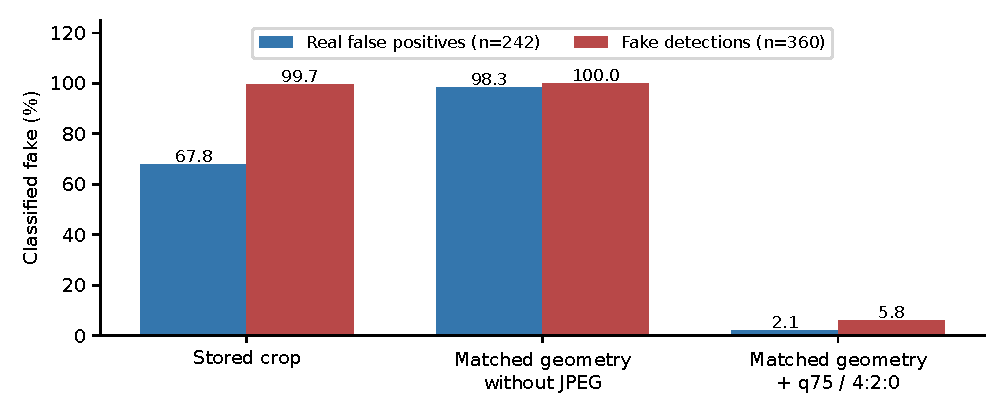
\includegraphics[width=\linewidth]{generated/processing_probe.pdf}
\caption{Existing validation-only diagnostic with frozen $L_A$ and threshold. A matched-geometry JPEG treatment
reduces real false positives but also erases much of the measured fake sensitivity. These transformed images
are diagnostic interventions, not validated authenticity-preserving demographic counterfactuals.}
\label{fig:probe}
\end{figure}

\Cref{fig:probe} summarizes three of the recorded processing arms. Geometry changes alone do not reproduce
the JPEG-associated drop: the matched-geometry lossless arm flags 98.3\% of the reals and 100\% of the fakes.
Adding quality-75, 4:2:0 processing lowers the corresponding rates to 2.1\% and 5.8\%.
The fake diagnostic contains 360 images across 24 methods. Thus the transformation cannot be interpreted
as a safe repair that preserves forgery evidence; it changes the detector's behavior on both classes.
Additional quality/subsampling probes are retained in the aggregate evidence.
These results support processing sensitivity and source confounding. They do not prove that compression
is the sole cause of every demographic disparity, or that the same mechanism holds for every model.

\section{Implemented Original-Image Pilot}
\subsection{Architecture and training scope}
The reported RF variants use one Xception encoder \cite{chollet2017}, global average pooling and one linear
real/fake head. They have 20,809,001 parameters, of which 6,790,433 are trainable under the exit-block policy:
6,788,384 encoder parameters and 2,049 head parameters. These figures come from the model's parameter report,
not from the larger global/local/gated CES-FL architecture used in some earlier project arms.
BatchNorm running statistics remain frozen. Trainable exit-block weights still receive gradients;
the encoder is not executed under \texttt{no\_grad} in this policy.

All six RF runs start from the same transferred FF2 BCE50 encoder, whose SHA256 begins
\texttt{741a8eb5b60a}. They differ in downstream seed or the declared augmentation.
Seeds 7, 17 and 27 therefore measure downstream variability conditional on one seed-17 encoder,
not the variability of independently repeated 50-epoch pretraining.
Each downstream run completes ten epochs. AdamW uses encoder/head learning rates $10^{-5}/10^{-3}$,
weight decay $10^{-4}$, batch size 32, and gradient-norm clipping at 5.
Images are converted to RGB, resized bilinearly to $224\times224$, and normalized by $(x-0.5)/0.5$.
Training uses bfloat16 autocast where configured; evaluation uses float32.

\subsection{Real false-alarm risk objective}
Every original TRAIN image appears in the classification stream once per epoch.
For observed class$\times$eight-group cells $c$, fixed weights are
$w_i=N/(|\mathcal C|n_{c(i)})$, giving mean weight one over TRAIN.
The classification objective is weighted binary cross entropy, $\mathcal L_{\rm cls}$.
Every fourth update adds a balanced real-image microbatch with 16 samples from each of the eight
gender$\times$race groups. Given TRAIN-derived threshold $t$ and temperature $\tau$, define
\begin{align}
 r_g &= \frac{1}{|\mathcal B_g|}\sum_{i\in\mathcal B_g}\sigma((z_i-t)/\tau),\\
 \bar r &= \sg\!\left[\sum_g\pi_g r_g\right],\\
 \mathcal L_{\rm rf} &= \frac{1}{|\mathcal G|}\sum_g|r_g-\bar r|.
 \label{eq:risk}
\end{align}
Here $\pi_g$ is the natural TRAIN-real group proportion. The detached reference prevents a direct gradient
through its calculation, but the absolute deviations remain \emph{two-sided}: low-risk groups can be pushed
upward. It is incorrect to describe this implementation as a one-sided upper-risk penalty.

On fairness events, the update uses
$\mathcal L_{\rm cls}+4\lambda\mathcal L_{\rm rf}$; other steps use classification only.
$\lambda$ ramps from zero to 0.1 over two epochs; $\tau$ decreases from 1 to 0.25 across the schedule.
The threshold is refreshed approximately four times per epoch from a fixed, seed-specific subset of 2,048
TRAIN real images. No SELECT or TEST images contribute gradients.
This surrogate approximates exceedance risk but does not guarantee equal hard FPR at the separately
calibrated SELECT threshold.

RF-S uses this objective without JPEG augmentation. RF-SJg adds a source-scale-emulated quality-75, 4:2:0
JPEG treatment to 15\% of classification-stream images, with the same rule for both labels and all groups.
The scale distribution is fixed from TRAIN FairFace-real crop scales. Auxiliary real microbatches remain
unmodified. No generated demographic edits, map-consistency terms, no-change-control losses, forensic
sensitivity loss or manipulation-response alignment terms are active in these RF experiments.

\subsection{Fixed checkpoint selection}
Among completed epochs satisfying SELECT AUC $\ge99.5$\% and SELECT FNR $\le0.5651$\%, selection minimizes
hard gender$\times$race $\ffpr$, then prefers higher AUC and the earlier epoch. The fairness metric is
not used to choose a different checkpoint after TEST.
Earlier stronger augmentation variants have no feasible checkpoint under these guards and are retained as
negative development results. The validation-driven exploration preceded the final frozen TEST checkpoint list;
the final three-seed repeats do not convert the whole development history into a single prospectively fixed design.

\section{Results}
\subsection{Validation and held-out results}
The six selected RF checkpoints and their epochs are listed in the appendix. RF-S achieves
SELECT $100\ffpr=34.24\pm0.21$ and RF-SJg $29.03\pm1.71$, with AUC near 99.80\% and 99.76\%, respectively.
These are SELECT development results, not substitutes for TEST performance.

\begin{table*}[t]
\centering\small
\begin{tabular}{lcrrrrr}
\toprule
Method & $n$ & AUC$\uparrow$ & FPR$\downarrow$ & FNR$\downarrow$ & $100F_{\rm FPR}\downarrow$ & WG-AUC$\uparrow$ \\
\midrule
Corrected GDA$^\dagger$ & 1 & 93.08 & 11.38 & 7.80 & 9.47 & 89.03 \\
DAW-FDD$^\dagger$ & 1 & 98.87 & 14.41 & 2.29 & 45.35 & 97.22 \\
CES-FL P$^\dagger$ & 1 & 98.78 & 12.39 & 2.92 & 42.23 & 96.85 \\
$L_A$ (BCE) & 1 & 99.00 & 15.14 & 1.44 & 63.67 & 97.33 \\
RF-S & 3 & $98.98 \pm 0.01$ & $14.92 \pm 0.16$ & $1.60 \pm 0.13$ & $60.95 \pm 1.92$ & $97.28 \pm 0.02$ \\
RF-SJg & 3 & $98.60 \pm 0.06$ & $13.69 \pm 0.28$ & $2.84 \pm 0.26$ & $47.69 \pm 3.91$ & $96.43 \pm 0.16$ \\
\bottomrule
\end{tabular}

\caption{Existing frozen FairForge-2 TEST evaluation, gender$\times$race axis. Rates and AUC are multiplied by 100;
$100\ffpr$ is a summed disparity. $n$ counts downstream seeds. $\pm$ is sample SD, not a confidence interval.
$\dagger$ marks local comparator implementations with distinct training/selection budgets; corrected GDA is
not the original published Ding result. Worst-group AUC uses eight eligible groups.}
\label{tab:test}
\end{table*}

\begin{figure}[t]
\centering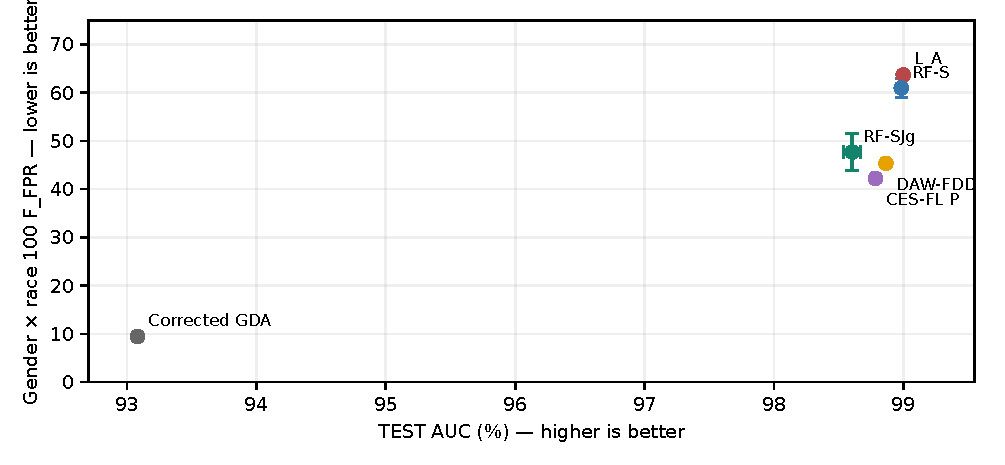
\includegraphics[width=\linewidth]{generated/test_tradeoff.pdf}
\caption{TEST utility/disparity trade-off. Bars show downstream seed SD for RF-S and RF-SJg; singleton methods
have no estimated training-seed variability. Differences in training/selection budgets limit causal comparisons
across method families.}
\label{fig:tradeoff}
\end{figure}

On TEST (\cref{tab:test}), RF-SJg lowers mean $100\ffpr$ by 13.26 points relative to RF-S, a descriptive
21.8\% reduction. All three matched downstream-seed differences have this direction.
The change costs about 0.38 AUC percentage points and increases FNR. Achieved overall FPR also differs across
methods, despite a common requested SELECT target of 10\%.
These observations establish a trade-off, not Pareto dominance or a significant improvement under a
contributor-aware confidence interval, which is not yet available.

RF-SJg does not outperform the local corrected GDA on the primary disparity and does not outperform
DAW-FDD on both AUC and disparity. The corrected GDA has TEST AUC 93.08\% and $100\ffpr=9.47$;
RF-SJg has 98.60\% and 47.69. Neither an overall superiority claim nor a claim of matching Ding's
published benchmark protocol follows from this comparison.

\subsection{Multiple axes and subgroup support}
\Cref{tab:axes} reports all supported demographic views without selecting favorable axes.
The primary gender$\times$race gain does not imply an improvement in gender, age or skin fairness;
some of these metrics worsen relative to RF-S. The same applies to detection and worst-group AUC.
The public CSVs include each seed, FPR/FNR, group support and additional disparity metrics.
The age$\times$skin axis is exploratory and depends on estimated labels.

\begin{table*}[t]
\centering\small
\begin{tabular}{lrrrrrr}
\toprule
Axis & GDA$^\dagger$ & DAW$^\dagger$ & P$^\dagger$ & $L_A$ & RF-S & RF-SJg \\
\midrule
Gender & 0.36 & 2.72 & 2.50 & 4.02 & $4.16 \pm 0.22$ & $4.36 \pm 0.13$ \\
Race & 3.29 & 22.24 & 20.42 & 31.15 & $29.70 \pm 1.05$ & $22.91 \pm 1.99$ \\
Gender $\times$ race & 9.47 & 45.35 & 42.23 & 63.67 & $60.95 \pm 1.92$ & $47.69 \pm 3.91$ \\
Age (estimated) & 4.37 & 12.53 & 8.17 & 13.25 & $12.71 \pm 0.79$ & $13.28 \pm 0.73$ \\
Skin (estimated) & 3.44 & 16.86 & 16.55 & 21.80 & $20.72 \pm 1.08$ & $14.83 \pm 0.33$ \\
Age $\times$ skin & 31.97 & 91.00 & 80.49 & 102.75 & $98.58 \pm 3.98$ & $86.00 \pm 2.18$ \\
Sex $\times$ age $\times$ race & 12.86 & 62.90 & 33.12 & 57.26 & $54.78 \pm 3.13$ & $53.74 \pm 2.79$ \\
\bottomrule
\end{tabular}

\caption{TEST $100\ffpr$ by axis. Age and skin labels are estimates. All displayed groups meet 20 images per class.
The number of groups differs by row, so magnitudes across rows are not directly comparable.
No per-metric seed or model oracle is used.}
\label{tab:axes}
\end{table*}

The gender$\times$race group supports are in the appendix. An image-level sample count must not be equated
with an independent-person count. Source identities and contributor clusters can yield substantially less
effective information. We therefore do not attach image-i.i.d. significance claims to small subgroup changes.
The existing processing probe's image bootstrap is likewise not a substitute for a contributor-aware interval.

\section{Provenance and Limitations}
\paragraph{Evaluation freeze and numerical replay.}
The recorded freeze lists four singleton checkpoints and two three-seed families: ten checkpoints in total;
one historical sentence mistakenly says nine. The current audit verifies checkpoint bytes, manifest hashes,
selected RF epochs, configuration digests and unchanged RF thresholds against aggregate receipts.
It does not rerun inference. The exporter family checks reproduced SELECT exactly for $L_A$ and P;
DAW and corrected GDA retained small metric differences under a revised validation-only tolerance
(AUC difference below $10^{-4}$; maximum fraction-unit metric difference below 0.015).
Near-threshold prediction flips were recorded. Their precise numerical cause is not independently established
by this audit; mixed-precision training alone does not prove it.

The freeze draft is recorded at commit \texttt{8d06aa09}; the final exported aggregate record is
\texttt{30a6b263}. Node/login clocks differ by roughly eleven minutes, so recorded timestamps alone do not
independently establish the claimed push-before-first-TEST-read order. Checkpoint paths are frozen in the
document, but pre-export checkpoint hashes are not all committed there. This temporal/provenance limitation
must be resolved before stronger preregistration claims. No new TEST inference or post-TEST training was
performed for this manuscript.

\paragraph{Duplicate run and compute.}
Two seed-7 RF-SJg runs exist. Their selected validation metrics are identical but checkpoint bytes differ.
This report uses the run in the existing TEST freeze for both SELECT and TEST, rather than choosing after
seeing outcomes. The second run is disclosed and charged as duplicate compute, not an additional seed.
The shared 72-GPU-hour ledger records 64.6011 GPU-hours charged and no active reservation at the audit time.
TEST/sanity inference durations are not fully reconciled, so 7.3989 hours is only the recorded ledger balance,
not proof of a complete all-study compute accounting. The shared ledger covers other work as well.

\paragraph{Evidence still missing.}
A full source/contributor-cluster uncertainty analysis, independently reviewed demographic annotations,
and a complete split-provenance audit remain necessary. Synthetic edit validity, complete counterfactual
training and cross-domain generalization of the final RF variants have not been established.
The single-seed local baseline adaptations use different budgets and selection policies. Historical
FF++/ResNet experiments and best-cell oracle tables must not be merged into the present model row.
The TEST set is now exposed; further development would require a new protected evaluation plan rather than
reusing its scores for tuning.

\section{Conclusion}
The current evidence shows that source-processing cues can strongly affect both demographic false alarms
and fake detection on FairForge-2. A controlled gentle-JPEG intervention improves the primary disparity
relative to its matched loss-only control across three downstream seeds, at a measurable utility cost.
It does not solve multi-axis fairness or establish superiority over the corrected local Ding comparator.
The next scientific step is to strengthen provenance, labels and uncertainty analysis while preserving the
frozen evidence, before making broader counterfactual or generalization claims.

{\small\bibliographystyle{ieeenat_fullname}\bibliography{references}}

\clearpage
\appendix
\section{Selected Checkpoints and Reproducibility}
\begin{table}[h]
\centering\small
\begin{tabular}{lcrrrr}
\toprule
Method & Seed & Epoch & AUC$\uparrow$ & FNR$\downarrow$ & $100F_{\rm FPR}\downarrow$ \\
\midrule
RF-S & 17 & 2 & 99.8032 & 0.2930 & 34.1222 \\
RF-S & 27 & 2 & 99.8079 & 0.3000 & 34.1222 \\
RF-S & 7 & 2 & 99.7993 & 0.2756 & 34.4818 \\
RF-SJg & 17 & 2 & 99.7549 & 0.4500 & 27.5259 \\
RF-SJg & 27 & 6 & 99.7514 & 0.5058 & 28.6686 \\
RF-SJg & 7 & 2 & 99.7603 & 0.4465 & 30.8859 \\
\bottomrule
\end{tabular}

\caption{Selected SELECT results from the exact checkpoints in the recorded TEST freeze. Every run completed
ten epochs. Different selected epochs reflect the fixed feasibility/selection rule, not unequal planned budgets.}
\end{table}

\begin{table}[h]
\centering\small\begin{tabular}{lrr}
\toprule
Gender $\times$ race & Real & Fake \\
\midrule
Female-Asian & 449 & 8711 \\
Male-Asian & 722 & 11573 \\
Female-Black & 475 & 8392 \\
Male-Black & 585 & 10261 \\
Female-White & 567 & 9348 \\
Male-White & 612 & 10654 \\
Female-Others & 691 & 7961 \\
Male-Others & 1340 & 15223 \\
\bottomrule
\end{tabular}

\caption{TEST image counts shared by the evaluated checkpoints. These counts do not certify independent people.}
\end{table}

\begin{figure*}[t]
\centering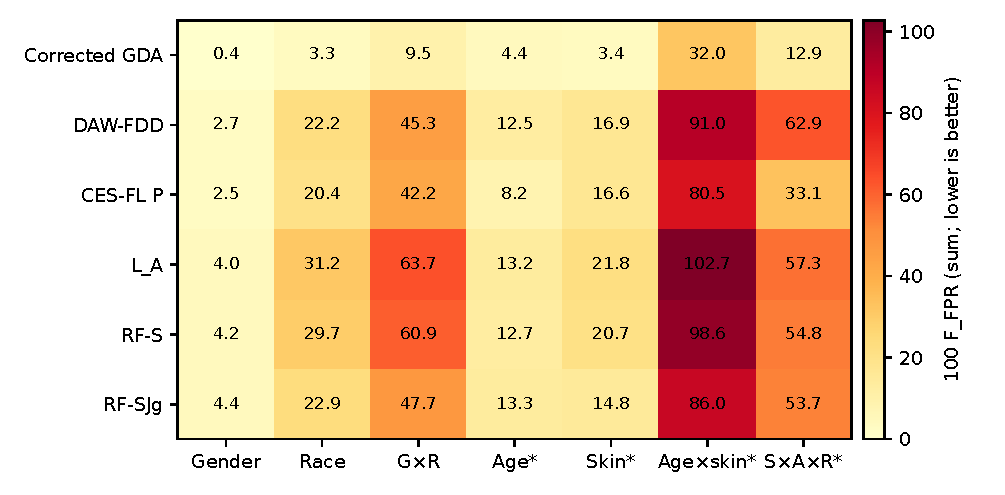
\includegraphics[width=.93\textwidth]{generated/test_fairness_axes.pdf}
\caption{All-axis TEST disparity overview (seed mean for RF families). Asterisks mark axes involving estimated
age/skin labels. Lower is better within a column; the sum has a different group count across columns.}
\end{figure*}

Public evidence is in \texttt{CES\_FL/paper/evidence/}. It contains aggregate metrics, group counts,
configuration/source/checkpoint hashes and training-epoch summaries. It excludes face images, checkpoints,
private reviews and individual prediction rows. The build scripts access only committed aggregates; no
training, inference or cluster connection is part of manuscript compilation.

The audited upstream scientific/result commit is
\texttt{30a6b263aaa63677cf8d3d9f4ee51bdb472ae284}. RF-SJg scientific source SHA256 begins
\texttt{2d99295cc0b8190a}; the shared core begins \texttt{8c25ba8cb844b059}.
The unchanged pre-extension RF-S source is recorded separately in its receipts.
Exact complete hashes and cluster-only artifact paths are retained in the evidence index.
Reference metadata was checked against primary author/publisher pages on 9 November 2026.

\end{document}
